\documentclass[11pt,a4paper]{article}

\usepackage[margin=1in]{geometry}
\usepackage{amsmath,amssymb}
\usepackage{booktabs}
\usepackage{tabularx}
\usepackage{graphicx}
\usepackage{subcaption}
\usepackage{xcolor}
\usepackage{microtype}
\usepackage[colorlinks=true,linkcolor=blue,citecolor=blue,urlcolor=blue]{hyperref}
\usepackage{algorithm}
\usepackage{algpseudocode}
\usepackage{natbib}
\bibliographystyle{plainnat}

\newcommand{\ReportedSpeedupKThree}{1.5}
\newcommand{\CorrectedSpeedupKThree}{1.04}
\newcommand{\CorrectedSkipKThree}{1.10}
\newcommand{\WarmupBaseline}{140.6}
\newcommand{\MedianBaseline}{28.3}
\newcommand{\CallReductionKThree}{3.2}
\newcommand{\PsnrTaylorKOne}{20.8}
\newcommand{\PsnrSpecKOne}{18.9}
\newcommand{\SpeedupTaylorKOne}{1.08}
\newcommand{\SpeedupSpecKOne}{1.02}
\newcommand{\BestTaylorRelLTwo}{0.205}
\newcommand{\BestTaylorStep}{6}
\newcommand{\WalkerBest}{0.242}
\newcommand{\WalkerFinal}{0.257}
\newcommand{\InterpFinal}{0.298}
\newcommand{\TrainEpochs}{12}
\newcommand{\DegenerateRelLTwo}{5.48 \times 10^{9}}
\newcommand{\DegenerateStep}{14}


\newcommand{\relltwo}{\ensuremath{\mathrm{relL2}}}

\title{\textbf{Latent Teleportation}\\[0.3em]
\large Forecasting Diffusion Trajectories for Faster Image Generation\\
\large Methods, Ablations, and a Serving Bottleneck Study}

\author{Lee Penkman\\[0.2em]
\normalsize CuteDSL / OmniServe\\
\normalsize \texttt{leepenkman@gmail.com}}

\date{\today}

\begin{document}
\maketitle

\begin{abstract}
Speculative decoding accelerated autoregressive language models by exploiting a
structural accident: decoding one token reads the entire weight matrix, so
verifying several drafted tokens in one wider batch is nearly free. We ask
whether the analogous accident exists in diffusion sampling, where a denoising
step is likewise a single pass over a large transformer, and where the latent
trajectory is smooth enough that the next point along it looks eminently
guessable.

We evaluate two families of forecaster: a learned \emph{latent walker} with a
\emph{gap interpolator} that drafts $k$ cheap steps and teleports the draft onto
the big model's likely trajectory, and a training-free first-order Taylor
extrapolation of the trajectory's own momentum, in the spirit of
TaylorSeer \citep{liu2025taylorseer}. We additionally implement a
$k$-nearest-neighbour trajectory cache and confidence-gating machinery, but do
not include them in the end-to-end claims: those components remain system
designs until they receive the same controlled image evaluation.

The main result has two parts. First, the signal is real: diffusion trajectories
are highly forecastable, and a schedule-calibrated momentum rule reduces
held-out trajectory error by 20--33\% over first-order Taylor across horizons
$k=1\ldots4$. Across the 36 evaluated learned and Taylor image candidates, an
author screen finds that every output retains the requested subject or scene;
the visible trade is increasing layout and texture drift as $k$ grows. Second,
the present serving point does not yet turn fewer denoiser calls into a large
end-to-end gain. At $512^2$ and 16 steps on an RTX 5090, speculative walking
reaches $\CorrectedSpeedupKThree\times$, while a destructive skip control that
removes $\CallReductionKThree\times$ of the denoiser reaches only
$\CorrectedSkipKThree\times$. This locates the immediate bottleneck in timed
text encoding and VAE decoding, and gives the next experiments a concrete
target rather than closing the direction.

We further report that our first analysis of these same runs claimed
$\ReportedSpeedupKThree\times$, and that this figure was an artifact of an
un-warmed first iteration whose baseline took $\WarmupBaseline$\,s against a
$\MedianBaseline$\,s median. We give the corrected protocol, a reproducible
analysis harness, five-fold forecaster ablations, draft-length and routing
ablations, three grids
containing the actual generated images across six prompt/style slices, an
account of how the method extends to swarms of LoRA adapters with disjoint
embedding spaces, and deployment recommendations grounded in the measured
speed--quality frontier.
\end{abstract}

\section{Introduction}

A diffusion sampler spends nearly all of its arithmetic evaluating one large
denoiser many times over. The obvious economy is to evaluate it fewer times, and
the literature offers two broad routes: change the model so that fewer steps
suffice --- distillation \citep{salimans2022progressive}, consistency models
\citep{song2023consistency,luo2023lcm}, adversarial distillation
\citep{sauer2023adversarial} --- or leave the model alone and reuse computation
across steps \citep{ma2024deepcache,selvaraju2024fora,liu2025taylorseer}. The
second route is attractive operationally because it does not require retraining
a production checkpoint.

Speculative decoding \citep{leviathan2023speculative,chen2023accelerating}
suggests a third framing. In language models, the win comes not from a better
model but from a hardware fact: autoregressive decode is memory-bandwidth-bound,
so a batch of $k+1$ candidate tokens costs about what one costs, and a cheap
drafter can propose tokens that the real model merely \emph{verifies}. The
appeal is that verification is exact --- the accepted output is distributed
exactly as the target model's --- so speculation is a pure latency optimisation
rather than a quality trade.

Diffusion sampling looks superficially similar. It is iterative, each iteration
is one pass over a transformer, and the sequence of latents
$x_0, x_1, \dots, x_N$ is a smooth curve rather than a sequence of discrete
symbols --- if anything, easier to extrapolate than text. This paper asks
which parts of the analogy carry, which do not, and what must change for the
forecastability signal to become useful serving latency.

\subsection*{What latent teleportation is --- and is not}

The name describes a family of approximate trajectory shortcuts, not one fixed
algorithm and not an exact analogue of language-model speculative decoding.

\begin{center}
\small
\begin{tabularx}{\textwidth}{@{}>{\raggedright\arraybackslash}X>{\raggedright\arraybackslash}X@{}}
\toprule
\textbf{What it is} & \textbf{What it is not} \\
\midrule
A forecast or warm start in a continuous diffusion latent trajectory. & An exact verifier or a distribution-preserving decoding method. \\
A family that can use momentum, learned predictors, confidence gates, or retrieved trajectories. & A claim that every listed mechanism has already passed image and latency evaluation. \\
A controllable trade between denoiser calls and same-seed image retention. & A guarantee of end-to-end speedup when text, VAE, transfer, or scheduling costs dominate. \\
A model--serving co-design problem whose useful operating point can change with resolution, schedule, and batching. & A single checkpoint-specific result that should be extrapolated to every sampler or deployment. \\
\bottomrule
\end{tabularx}
\end{center}

\paragraph{Contributions.}
\begin{enumerate}
  \item \textbf{A predictability study} of the Z-Image \citep{zimage2025} latent
    trajectory: a $(t,k)$ grid of forecast error for identity, first-order
    Taylor and scalar-affine predictors, establishing that the trajectory is
    genuinely forecastable and quantifying where (Section~\ref{sec:gap}).
  \item \textbf{A five-fold forecaster ablation} showing that one fitted
    schedule scalar improves over raw Taylor by 20--33\%, while an extra
    historical delta adds little and an unfitted second-order rule is worse
    (Section~\ref{sec:calibration}).
  \item \textbf{Two evaluated acceleration mechanisms} --- speculative latent
    walking with a learned gap interpolator and fixed-horizon Taylor forecasting
    --- plus clearly separated designs for confidence gating and $k$-NN cache
    teleportation (Section~\ref{sec:method}).
  \item \textbf{An operating-point bottleneck diagnosis}: call reductions
    of $\CallReductionKThree\times$ yield $\CorrectedSpeedupKThree\times$
    wall-clock, and a skip-everything ablation caps at
    $\CorrectedSkipKThree\times$, localising the bottleneck outside the
    denoiser (Section~\ref{sec:e2e}).
  \item \textbf{A methodological correction}. Our own earlier reading of these
    runs reported $\ReportedSpeedupKThree\times$; we show it was warm-up
    contamination, and ship an analysis harness that cannot make that mistake
    again (Section~\ref{sec:correction}).
  \item \textbf{Image-level ablations} over learned speculation, Taylor
    forecasting, a destructive skip control, three draft lengths, and six
    prompt/style slices. We publish all panels as contact sheets with PSNR,
    SSIM, and source-file hashes (Section~\ref{sec:image-ablations}).
  \item \textbf{An extension sketch to LoRA armies}, where adapters induce
    disjoint latent statistics and a shared trajectory cache needs an embedding
    normalisation network (Section~\ref{sec:lora}).
\end{enumerate}

\section{Background and Related Work}

\paragraph{Diffusion and flow samplers.}
We work with a rectified-flow / flow-matching formulation
\citep{liu2023rectified,lipman2023flow} as used by Z-Image, sampled on a fixed
schedule of $N$ timesteps in a latent space produced by a VAE
\citep{rombach2022ldm}, with a DiT-style denoiser \citep{peebles2023dit}.
Writing $\Phi$ for one scheduler step,
\begin{equation}
  x_{i+1} = \Phi(x_i, t_i, c),
\end{equation}
with $c$ the text conditioning. The cost of sampling is $N$ evaluations of the
denoiser inside $\Phi$, plus one text encode and one VAE decode.

\paragraph{Step reduction by retraining.}
Progressive distillation \citep{salimans2022progressive}, consistency models
\citep{song2023consistency}, latent consistency models \citep{luo2023lcm} and
adversarial distillation \citep{sauer2023adversarial} all produce a new
checkpoint that needs fewer steps. These are the strongest known accelerations
and are orthogonal to our work; Z-Image Turbo is already a few-step model, which
matters for interpreting our results (Section~\ref{sec:limitations}).

\paragraph{Training-free caching.}
DeepCache \citep{ma2024deepcache} reuses U-Net skip features across adjacent
steps. FORA \citep{selvaraju2024fora} caches attention and MLP outputs in
diffusion transformers. TaylorSeer \citep{liu2025taylorseer} --- the line our
codebase calls CG-Taylor --- reframes caching as \emph{forecasting}: rather than
reusing a stale feature, extrapolate it with a Taylor series in the timestep
index. Crucially, these methods are fitted to a specific model: the cache
schedule and the expansion order are tuned per checkpoint, and transfer is not
claimed. Our approach inherits that property and we make it explicit, since it
is a real deployment cost rather than an incidental detail.

\paragraph{Speculative decoding.}
Draft-and-verify \citep{leviathan2023speculative,chen2023accelerating}, with
later variants that avoid a separate draft model by adding heads
\citep{cai2024medusa}, reusing features \citep{li2024eagle}, or drafting from
the prompt itself \citep{saxena2023promptlookup}. The property that makes these
work is verification: the target model's distribution is preserved exactly. It
is worth stating plainly that \emph{our diffusion analogue does not have this
property}. There is no cheap exact verifier for ``is this latent the one the big
model would have produced'', so every method in this paper is an approximation
with a quality cost, and must be evaluated as such.

\section{Method}
\label{sec:method}

\subsection{Speculative latent walking}

The drafting scheme mirrors speculative decoding structurally. The big model
takes one real step; a small network drafts the next $k$; a second network
corrects the endpoint of the draft onto where the big model's trajectory would
plausibly have gone; the loop resumes with a real step.

The \textbf{latent walker} $W$ predicts the next latent from the current one and
the trajectory's momentum $\delta_i = x_i - x_{i-1}$:
\begin{equation}
  \hat{x}_{i+1} = x_i + \delta_i + W(x_i, \delta_i, t_i),
\end{equation}
so that the network learns only the \emph{correction} to constant-velocity
motion. The output convolution is zero-initialised, making the network exactly a
momentum extrapolator at initialisation and guaranteeing it starts no worse than
the training-free baseline. Rolling $W$ out $k$ times, feeding it its own
predicted movement, yields a draft endpoint $\hat{x}_{i+k}$.

The \textbf{gap interpolator} $G$ then teleports that endpoint:
\begin{equation}
  \tilde{x}_{i+k} = \hat{x}_{i+k} + G(x_i, \delta_i, \hat{x}_{i+k}, t_i, k),
\end{equation}
again residual and zero-initialised, so identity means ``trust the walker''. Both
networks are small FiLM-conditioned residual CNNs operating directly on the
$16$-channel latent, conditioned on sinusoidal embeddings of the fractional
timestep and the schedule length.

\subsection{First-order Taylor forecasting and confidence gating}

The training-free baseline extrapolates the trajectory's own momentum:
\begin{equation}
  \tilde{x}_{i+k} = x_i + k\,(x_i - x_{i-1}),
  \label{eq:taylor}
\end{equation}
which is exactly a first-order Taylor step in the step index, in the spirit of
\citet{liu2025taylorseer}. This is the floor every learned method must beat, and
in our results it is a stubbornly high floor.

The \textbf{confidence gate} would add the CG in CG-Taylor. Rather than a fixed
skip schedule, it tracks the recent history of prediction error, estimates the
derivative of that error, and maps the resulting confidence onto a number of
refinement steps to spend --- high confidence, fewer real steps. The design
intent is the diffusion analogue of forecasting one block into the network and
committing to the whole step if that forecast lands: a cheap partial computation
acts as a proxy for whether the expensive full computation can be skipped. The
end-to-end Taylor arm reported below uses fixed $k$ and does not activate this
gate; we therefore treat confidence gating as unvalidated system design.

\subsection{Latent teleportation from a trajectory cache}

The third mechanism drops speculation entirely and asks a different question:
if this prompt resembles one we have generated before, can we start from where
that generation \emph{ended up} rather than from noise?

The cache stores, per generation, the full sequence of intermediate latents
together with a CLIP \citep{radford2021clip} embedding of the prompt and a
tokenisation of it into \emph{visual units} --- noun-phrase-like fragments that
recur across prompts --- plus bigrams of adjacent units. At query time the
system retrieves the $k$ nearest cached trajectories by prompt embedding,
combines their latents at a chosen injection timestep (SLERP, a learned
combiner, or a tree combiner), injects the result, and runs only the remaining
scheduler steps. A $k$-NN \emph{trajectory prior} additionally warm-starts the
walker rollout with neighbour deltas.

The intuition is that similar refinements trace similar paths through the latent
manifold, so a neighbourhood of finished trajectories defines a local chart that
a new generation can be teleported into. Storage is SafeTensors blobs indexed by
SQLite; retrieval is exact $k$-NN over a few thousand vectors, for which a
brute-force scan suffices and \citet{johnson2019faiss} would be the drop-in
replacement at scale.

\subsection{Extension to LoRA armies}
\label{sec:lora}

Production serving does not run one checkpoint. It runs a base model with a
library of LoRA adapters \citep{hu2022lora} swapped per request --- in our
deployment, an army of style and subject adapters, hot-swapped between
generations. This breaks the trajectory cache in a specific way: an adapter
shifts the latent statistics, so a trajectory collected under adapter $A$ is not
a valid warm start under adapter $B$, even for an identical prompt. Naively
sharing the cache produces exactly the failure mode the confidence gate is
supposed to catch, but at a magnitude that no gate rescues.

The extension we propose --- and have not yet validated, so we state it as
design rather than result --- is an \emph{embedding normalisation network}: a
small conditional map $\eta_{A \to B}$ trained to transport a latent from
adapter $A$'s trajectory space into adapter $B$'s, conditioned on both adapter
identities and the timestep. Cheap variants worth trying first, in increasing
order of capacity, are (i) per-adapter per-timestep channel-wise
mean/variance renormalisation, which costs two vectors per adapter per step;
(ii) a low-rank affine map fitted per adapter pair; (iii) a shared conditional
network taking learned adapter embeddings, which scales to $O(n)$ parameters
rather than $O(n^2)$ for $n$ adapters. Adapter identity is exactly the kind of
low-cardinality conditioning that FiLM handles well, and the zero-initialised
residual trick used above applies again: initialise to identity so that a shared
cache degrades to a per-adapter cache rather than to garbage.

The adapter library and its serving stack are not open-sourced; the mechanism
described here is, in \citet{cutedsl}.

\section{Experimental Setup}

All measurements are on a single RTX 5090 (32\,GB, sm\_120, compute capability
12.0) using Z-Image Turbo in \texttt{bfloat16}, at $512\times512$ with a 16-step
schedule and guidance 0, seed fixed at 7 across arms. Trajectory capture
collected 200 full 16-step trajectories (402\,MB) storing every intermediate
latent. The image ablation uses six deliberately heterogeneous prompt slices:
golden-hour landscape, dramatic portrait, snowy night, cyberpunk/neon,
soft-light wildlife, and isometric illustration. These labels describe prompt
content; they are not independent style datasets or LoRA adapters.

\paragraph{Metrics.} Forecast quality is measured by
\begin{equation}
  \relltwo = \frac{\lVert \tilde{x}_{i+k} - x_{i+k} \rVert_2}
                  {\lVert x_{i+k} - x_i \rVert_2},
\end{equation}
error normalised by how far the trajectory actually moved. This normalisation is
what makes the number interpretable: $\relltwo = 1.0$ is the score of predicting
no movement at all, so any method scoring near $1.0$ is worthless regardless of
its absolute error. End-to-end image agreement is PSNR against the full-schedule
baseline image. For the image grids we additionally report SSIM, computed on the
saved RGB PNGs. Both are reference-similarity metrics rather than measures of
prompt adherence or aesthetic quality. Wall clock is measured with CUDA
synchronisation around each arm.

\paragraph{Reproducibility.} Timing and latent-forecast numbers are emitted by
\texttt{paper\_analysis.py} from raw result JSON. Image tables and grids are
emitted by \texttt{paper\_ablation\_grids.py} from the 72 saved PNGs.
The latter writes a manifest containing the SHA-256 digest, prompt index,
method, $k$, PSNR, and SSIM for every source panel. No panel is synthesized or
retouched; grid construction is limited to resizing, borders, and labels.

\section{Results}

\subsection{The latent trajectory is forecastable}
\label{sec:gap}

Table~\ref{tab:gap} summarises the $(t,k)$ grid of forecast error. Two facts
stand out. First, first-order Taylor extrapolation is strong: at $k=1$ it
reaches $\relltwo = \BestTaylorRelLTwo$ around step $\BestTaylorStep$, meaning
the residual error is about a fifth of the movement being predicted. Second, the
scalar-affine predictor sits near $0.88$ --- barely better than not moving --- which
tells us the trajectory's predictability is genuinely directional rather than a
matter of getting the step size right.

\begin{table}[ht]
\centering
\begin{tabular}{rrrrr}
\toprule
$k$ & mean relL2 (taylor1) & best cell & mean relL2 (affine) & cells \\
\midrule
1 & 0.240 & 0.205 & 0.880 & 13 \\
2 & 0.318 & 0.255 & 0.879 & 13 \\
3 & 0.330 & 0.261 & 0.883 & 12 \\
4 & 0.369 & 0.261 & 0.880 & 11 \\
\bottomrule
\end{tabular}

\caption{Trajectory predictability by draft length. \relltwo{} is error over
actual movement; $1.0$ is the no-movement baseline. Lower is better. The
degenerate final-step cell is excluded (see text).}
\label{tab:gap}
\end{table}

Error degrades monotonically with $k$, as expected, and is worst at both ends of
the schedule: early steps move erratically, and the last scheduler step of this
16-step configuration moves the latent by approximately zero. That final step is
not merely hard to predict --- it is a no-op, and dividing by its movement
produced an \relltwo{} of $\DegenerateRelLTwo$ at $t=\DegenerateStep$. We exclude
that cell from all aggregates. In the stored float16 trajectories, the final
latent is duplicated; for this exact pipeline and schedule, that step is a
candidate for exact removal after verifying the duplication at runtime.

\subsection{Learned walker versus training-free Taylor}

Training the walker and interpolator for $\TrainEpochs$ epochs on the 200
captured trajectories reaches a best \relltwo{} of $\WalkerBest$ for the walker,
against roughly $0.21$--$0.30$ for Taylor over the comparable window --- an
improvement of order 15--20\% on the metric it was trained for. Momentum
conditioning is what produces this; an earlier position-only walker plateaued
around $0.6$, worse than Taylor.

The training is not clean, and we report it rather than presenting the best
epoch as if it were the endpoint. The walker's final-epoch score is
$\WalkerFinal$ and the interpolator's is $\InterpFinal$, both worse than their
best; a run that saves the last checkpoint therefore ships a model worse than
the one it trained. Any redeployment of this method should select on validation
\relltwo{} rather than take the final epoch.

\subsection{Schedule calibration improves the cheap forecaster}
\label{sec:calibration}

The basic Taylor rule assumes that one recorded movement should be multiplied
by exactly $k$. Diffusion schedules are not uniform in trajectory distance, so
we fit a separate scalar $\alpha_{t,k}$ for each step and horizon:
\begin{equation}
  \hat{x}_{t+k}=x_t+\alpha_{t,k}\,k\,(x_t-x_{t-1}).
\end{equation}
We also test a two-delta fit
$x_t+a_{t,k}(x_t-x_{t-1})+b_{t,k}(x_{t-1}-x_{t-2})$, an average-velocity
rule, and a direct second-order Taylor extrapolation. Coefficients are fitted on
four folds and evaluated on the held-out fifth, rotating over all five folds of
the 200 captured trajectories. Cells whose target movement is below $10^{-4}$
are excluded by the same rule as Section~\ref{sec:gap}.

\begin{table}[ht]
\centering
\scriptsize
\begin{tabular}{@{}crrrrr@{}}
\toprule
$k$ & Taylor-1 & avg. velocity & Taylor-2 & scaled momentum & two-delta fit \\
\midrule
1 & 0.221$\pm$0.005 & 0.273$\pm$0.004 & 0.226$\pm$0.009 & 0.176$\pm$0.007 & 0.172$\pm$0.007 \\
2 & 0.306$\pm$0.004 & 0.338$\pm$0.004 & 0.370$\pm$0.011 & 0.205$\pm$0.007 & 0.201$\pm$0.007 \\
3 & 0.317$\pm$0.004 & 0.352$\pm$0.004 & 0.395$\pm$0.013 & 0.228$\pm$0.008 & 0.226$\pm$0.008 \\
4 & 0.357$\pm$0.004 & 0.393$\pm$0.004 & 0.446$\pm$0.016 & 0.250$\pm$0.009 & 0.248$\pm$0.008 \\
\bottomrule
\end{tabular}

\caption{Five-fold held-out \relltwo{} (mean $\pm$ standard deviation across
folds). Lower is better. Scaled momentum fits one schedule scalar;
two-delta fits two. No image pixels or timing labels enter the fit.}
\label{tab:forecaster-ablation}
\end{table}

Table~\ref{tab:forecaster-ablation} gives a constructive tuning result. Scaled
momentum reduces error by 20--33\% relative to first-order Taylor, and the
two-delta fit reduces it by 22--34\%. The second delta contributes only a small
increment, making the one-scalar rule the better first deployment candidate.
Average velocity and raw second-order Taylor are both worse than first order:
more history or a higher expansion order is not automatically better unless it
is calibrated to the schedule. This is a held-out latent-level result, not yet
an image-quality or latency claim; the next image sweep should promote scaled
momentum alongside the existing Taylor reference.

\subsection{End-to-end: locating the remaining latency}
\label{sec:e2e}

Table~\ref{tab:e2e} measures the current serving point. Across draft lengths $k \in
\{1,2,3\}$, corresponding to $9$, $6$ and $5$ real denoiser calls out of $16$,
measured speedup never exceeds $1.10\times$ and speculative walking specifically
never exceeds $\CorrectedSpeedupKThree\times$.

\begin{table}[ht]
\centering
\begin{tabular}{rrrrrrrrr}
\toprule
$k$ & big steps & call red. & \multicolumn{3}{c}{wall-clock speedup} & \multicolumn{3}{c}{PSNR vs baseline (dB)} \\
\cmidrule(lr){4-6}\cmidrule(lr){7-9}
 & & & spec & taylor & skip & spec & taylor & skip \\
\midrule
1 & 9 & 1.78$\times$ & 1.02 & 1.08 & 1.03 & 18.9 & 20.8 & 11.0 \\
2 & 6 & 2.67$\times$ & 1.03 & 1.03 & 1.04 & 18.0 & 17.9 & 9.3 \\
3 & 5 & 3.2$\times$ & 1.04 & 1.09 & 1.10 & 17.0 & 16.9 & 8.9 \\
\bottomrule
\end{tabular}

\caption{Draft-length ablation at $512^2$, 16 steps, 5 prompts per cell after
warm-up exclusion. ``call red.'' is the reduction in denoiser evaluations;
speedup is measured wall clock. \emph{skip} performs no correction at all and
therefore bounds what any drafting scheme can achieve in this harness.}
\label{tab:e2e}
\end{table}

The diagnostic is the \emph{skip} column. That arm discards
$\CallReductionKThree\times$ of the denoiser evaluations and replaces them with
nothing --- its PSNR of $8.9$\,dB confirms the output is destroyed --- and it still
only reaches $\CorrectedSkipKThree\times$. Its observed ceiling is therefore
about $1.10\times$ at this operating point, implying that roughly 90\% of the
measured time is outside the removed calls. Inspecting the harness confirms it: the timed
region wraps \texttt{zimage\_prepare} (text encoding) and \texttt{zimage\_decode}
(VAE decode) along with the sampling loop, and at $512^2$ with a 16-step Turbo
schedule those fixed costs dominate. This is Amdahl's law
\citep{amdahl1967validity} arriving exactly on schedule.

A second observation from Table~\ref{tab:e2e}: at $k=1$ the training-free Taylor
arm is both faster ($\SpeedupTaylorKOne\times$ vs $\SpeedupSpecKOne\times$) and
higher quality ($\PsnrTaylorKOne$\,dB vs $\PsnrSpecKOne$\,dB) than the learned
walker. The learned networks win on the latent metric they were trained for but
lose on same-seed pixel retention. This sets a useful tuning reference: Taylor
at $k=1$ is the current image-level baseline, and a learned replacement needs an
image-aligned objective and validation-based checkpoint selection to displace it.

\subsection{Image ablations across methods, styles, and draft lengths}
\label{sec:image-ablations}

The aggregate timing result is bottleneck-limited, and the images answer the
complementary question of \emph{how} each approximation changes the sample.
Figures~\ref{fig:method-style},
\ref{fig:draft-grid}, and~\ref{fig:skip-grid} expose the entire recorded image
sweep rather than one
favourable prompt. The raw store contains 72 PNGs: six prompts, four arms, and
three values of $k$. Because the baseline is regenerated identically for every
$k$, this corresponds to six unique references and 54 candidate outputs. The
figures include all six prompt slices, including the first timing row excluded
as a warm-up outlier; warm-up affects latency, not the already-saved image.

\begin{table}[H]
\centering
\small
\begin{tabular}{@{}crrrrrrr@{}}
\toprule
$k$ & real calls & \multicolumn{2}{c}{learned} & \multicolumn{2}{c}{Taylor} & \multicolumn{2}{c}{skip} \\
\cmidrule(lr){3-4}\cmidrule(lr){5-6}\cmidrule(l){7-8}
 & & PSNR & SSIM & PSNR & SSIM & PSNR & SSIM \\
\midrule
1 & 9 & 18.14 & 0.699 & 19.78 & 0.770 & 11.11 & 0.244 \\
2 & 6 & 17.28 & 0.662 & 17.29 & 0.637 & 9.35 & 0.182 \\
3 & 5 & 16.51 & 0.629 & 16.39 & 0.585 & 8.95 & 0.173 \\
\bottomrule
\end{tabular}

\caption{Image hyperparameter ablation over all six prompts. Values are mean
PSNR (dB) and SSIM against the same-seed 16-step reference. Unlike
Table~\ref{tab:e2e}, no row is removed because this table contains no timing
measurement. Higher is better.}
\label{tab:image-hyperparams}
\end{table}

Table~\ref{tab:image-hyperparams} gives three robust observations. First,
$k=1$ is the quality frontier: Taylor reaches 19.78\,dB/0.770 and the learned
method 18.14\,dB/0.699. Second, mean similarity falls as $k$ grows. Learned
SSIM moves $0.699\rightarrow0.662\rightarrow0.629$, while Taylor moves
$0.770\rightarrow0.637\rightarrow0.585$. Third, the skip control is not a
plausible alternative generation: even at $k=1$ it reaches only 0.244 SSIM and
visually collapses to coloured noise. It is useful only as the compute-saving
upper bound in Table~\ref{tab:e2e}.

The style-stratified $k=3$ numbers in Table~\ref{tab:image-styles} show why six
rows matter. Learned speculation is ahead of Taylor on portrait, snowy-night,
and isometric prompts; Taylor is ahead on landscape, cyberpunk, and wildlife by
PSNR. The ranking is therefore three against three rather than a universal
winner. Structural retention also varies widely: learned SSIM ranges from 0.500
on the snowy scene to 0.791 on the isometric illustration. These are descriptive
slices, not confidence intervals, but they rule out a claim that one forecaster
dominates across visual regimes.

\begin{table}[H]
\centering
\scriptsize
\begin{tabular}{@{}lrrrrrr@{}}
\toprule
style slice & \multicolumn{2}{c}{learned} & \multicolumn{2}{c}{Taylor} & \multicolumn{2}{c}{skip} \\
\cmidrule(lr){2-3}\cmidrule(lr){4-5}\cmidrule(l){6-7}
 & PSNR & SSIM & PSNR & SSIM & PSNR & SSIM \\
\midrule
Golden-hour landscape & 13.87 & 0.713 & 14.12 & 0.666 & 9.32 & 0.165 \\
Dramatic portrait & 19.11 & 0.513 & 17.72 & 0.453 & 7.37 & 0.096 \\
Snowy night scene & 15.26 & 0.500 & 14.68 & 0.454 & 8.82 & 0.177 \\
Cyberpunk / neon & 14.70 & 0.504 & 15.74 & 0.506 & 9.33 & 0.217 \\
Soft-light wildlife & 18.53 & 0.751 & 18.82 & 0.692 & 11.79 & 0.284 \\
Isometric illustration & 17.61 & 0.791 & 17.28 & 0.738 & 7.08 & 0.097 \\
\bottomrule
\end{tabular}

\caption{Style-slice ablation at $k=3$ over the six recorded prompts. Each row
contains one image per method, so the values describe examples rather than a
population estimate.}
\label{tab:image-styles}
\end{table}

An oracle that independently chooses the higher-scoring learned or Taylor image
for each prompt estimates the available headroom from method routing. It is not
a deployable router because it sees the reference image and chooses PSNR and
SSIM independently.

\begin{table}[H]
\centering
\small
\begin{tabular}{@{}crrrrrr@{}}
\toprule
 & \multicolumn{3}{c}{PSNR (dB)} & \multicolumn{3}{c}{SSIM} \\
\cmidrule(lr){2-4}\cmidrule(l){5-7}
$k$ & learned & Taylor & oracle & learned & Taylor & oracle \\
\midrule
1 & 18.14 & 19.78 & 19.78 & 0.699 & 0.770 & 0.772 \\
2 & 17.28 & 17.29 & 17.62 & 0.662 & 0.637 & 0.665 \\
3 & 16.51 & 16.39 & 16.78 & 0.629 & 0.585 & 0.629 \\
\bottomrule
\end{tabular}

\caption{Reference-aware oracle routing between the learned and Taylor
candidates. The oracle is an unavailable upper bound, not an evaluated routing
algorithm. Higher is better.}
\label{tab:image-router}
\end{table}

Table~\ref{tab:image-router} shows modest routing headroom. At $k=1$, Taylor
already wins PSNR on every prompt; at $k=2$ and $k=3$, oracle selection adds
only 0.33 and 0.38 dB over the better fixed method. Oracle SSIM is similarly
close to the best fixed choice. Schedule calibration is therefore the more
promising immediate experiment; a learned router becomes worthwhile only when
the candidate methods are more complementary.

The grids also sharpen the metric caveat. A coherent candidate that moves a
subject or changes texture can score poorly against the reference, while SSIM
rewards structurally simple scenes differently from detailed photographs. We
therefore use these metrics to quantify same-seed retention, not to assert equal
aesthetic quality. A blinded human or calibrated vision-language preference
study remains required for that claim.

We additionally inspected every full-resolution source panel, not only the
contact sheets. In this unblinded author screen, all 36 learned and Taylor
candidates retained the requested subject or scene, with no catastrophic
collapse; increasing $k$ primarily introduced texture, geometry, and layout
drift. None of the 18 skip candidates passed the same usable-image screen,
although several $k=1$ panels retained fragments of scene structure. This is a
failure-mode check, not a blinded aesthetic or prompt-adherence evaluation.

\begin{figure}[p]
\centering
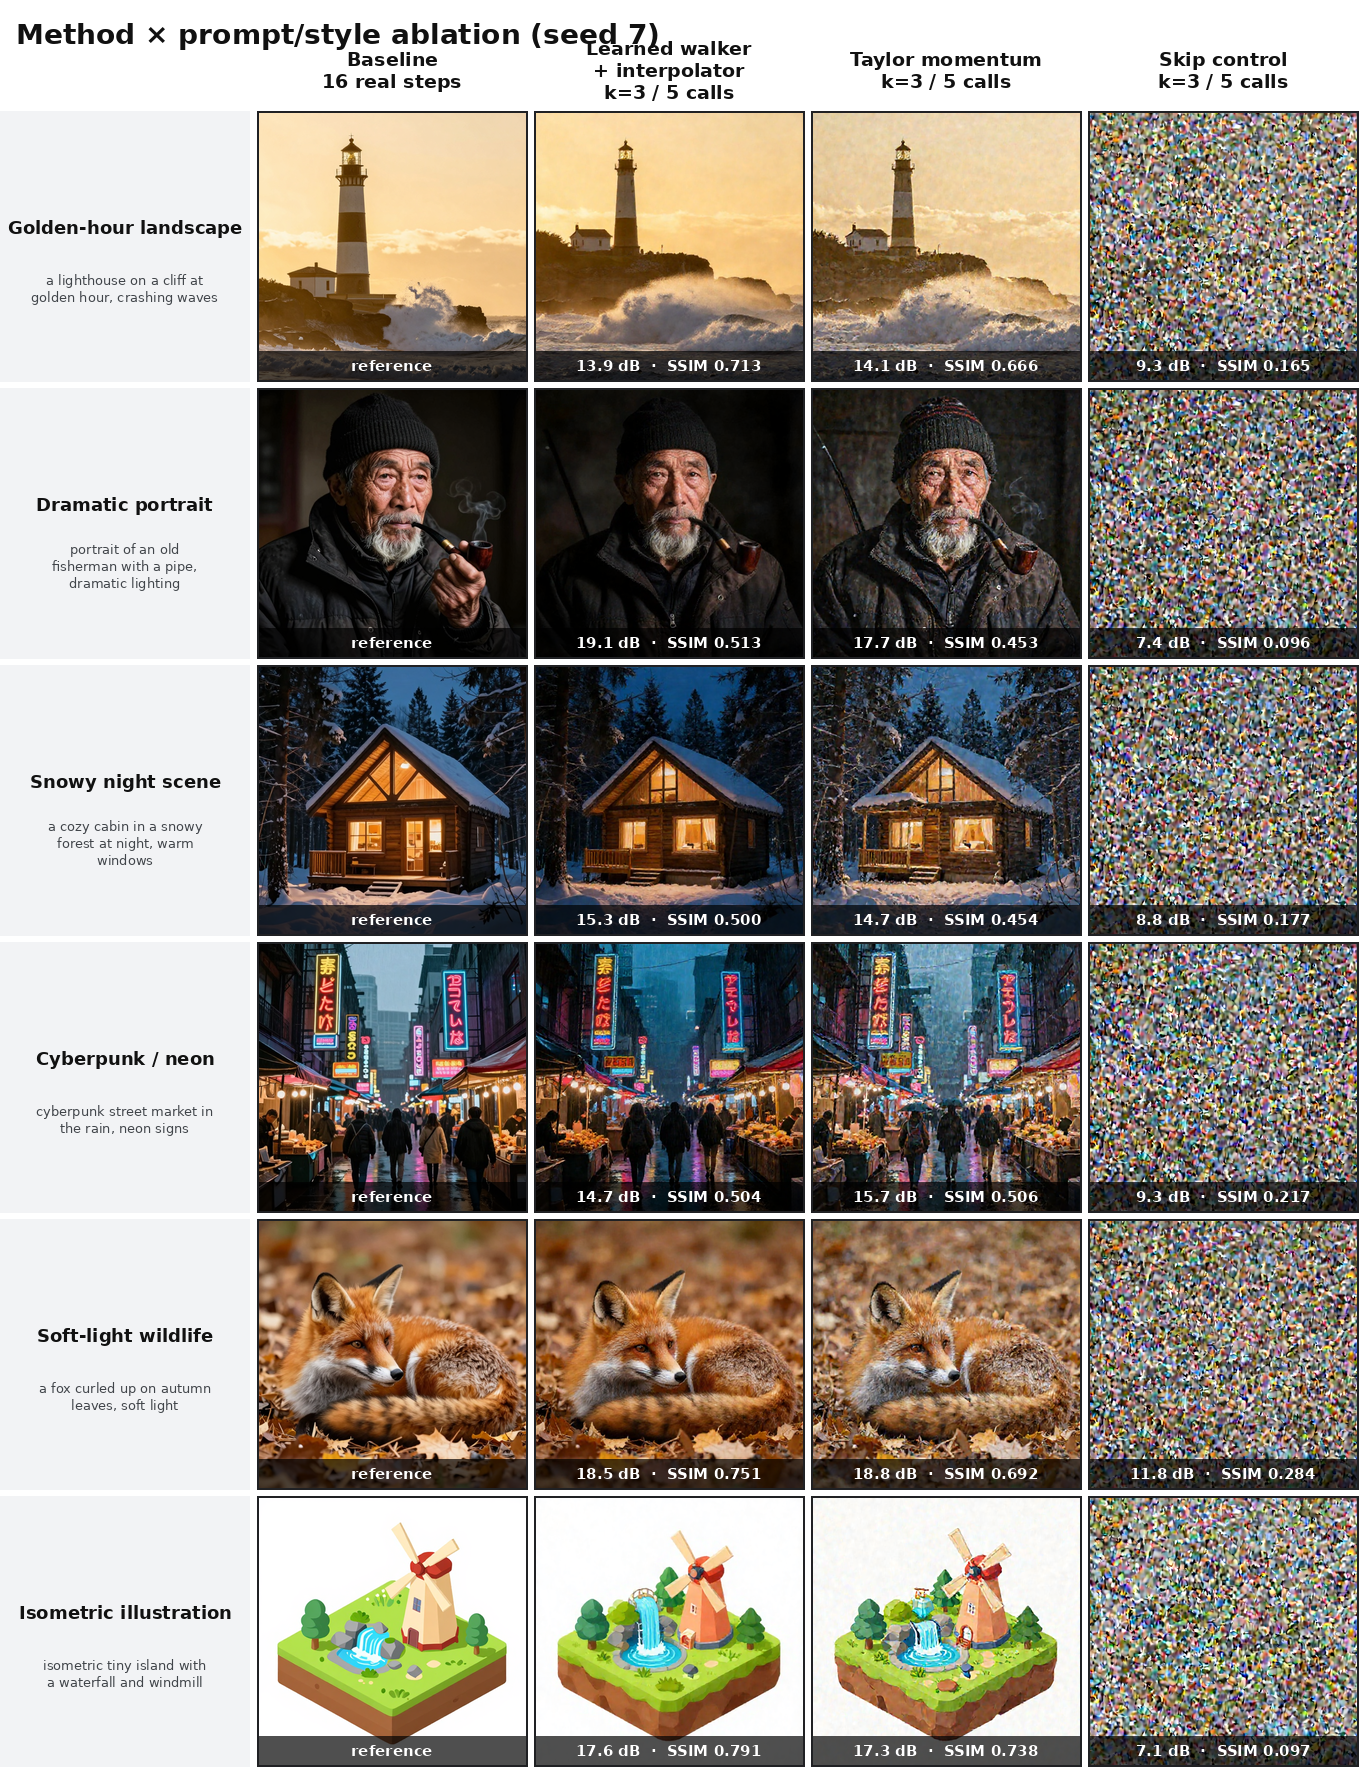
\includegraphics[width=\textwidth]{figures/method_style_grid.png}
\caption{Method $\times$ prompt/style ablation at $k=3$ (five real denoiser
calls), seed 7. Each row is one saved prompt; each panel is an actual generated
PNG with no content editing. The learned and Taylor arms usually preserve the
requested subject while changing layout, texture, or fine detail. The skip
control is visibly destructive in every slice.}
\label{fig:method-style}
\end{figure}

\begin{figure}[p]
\centering
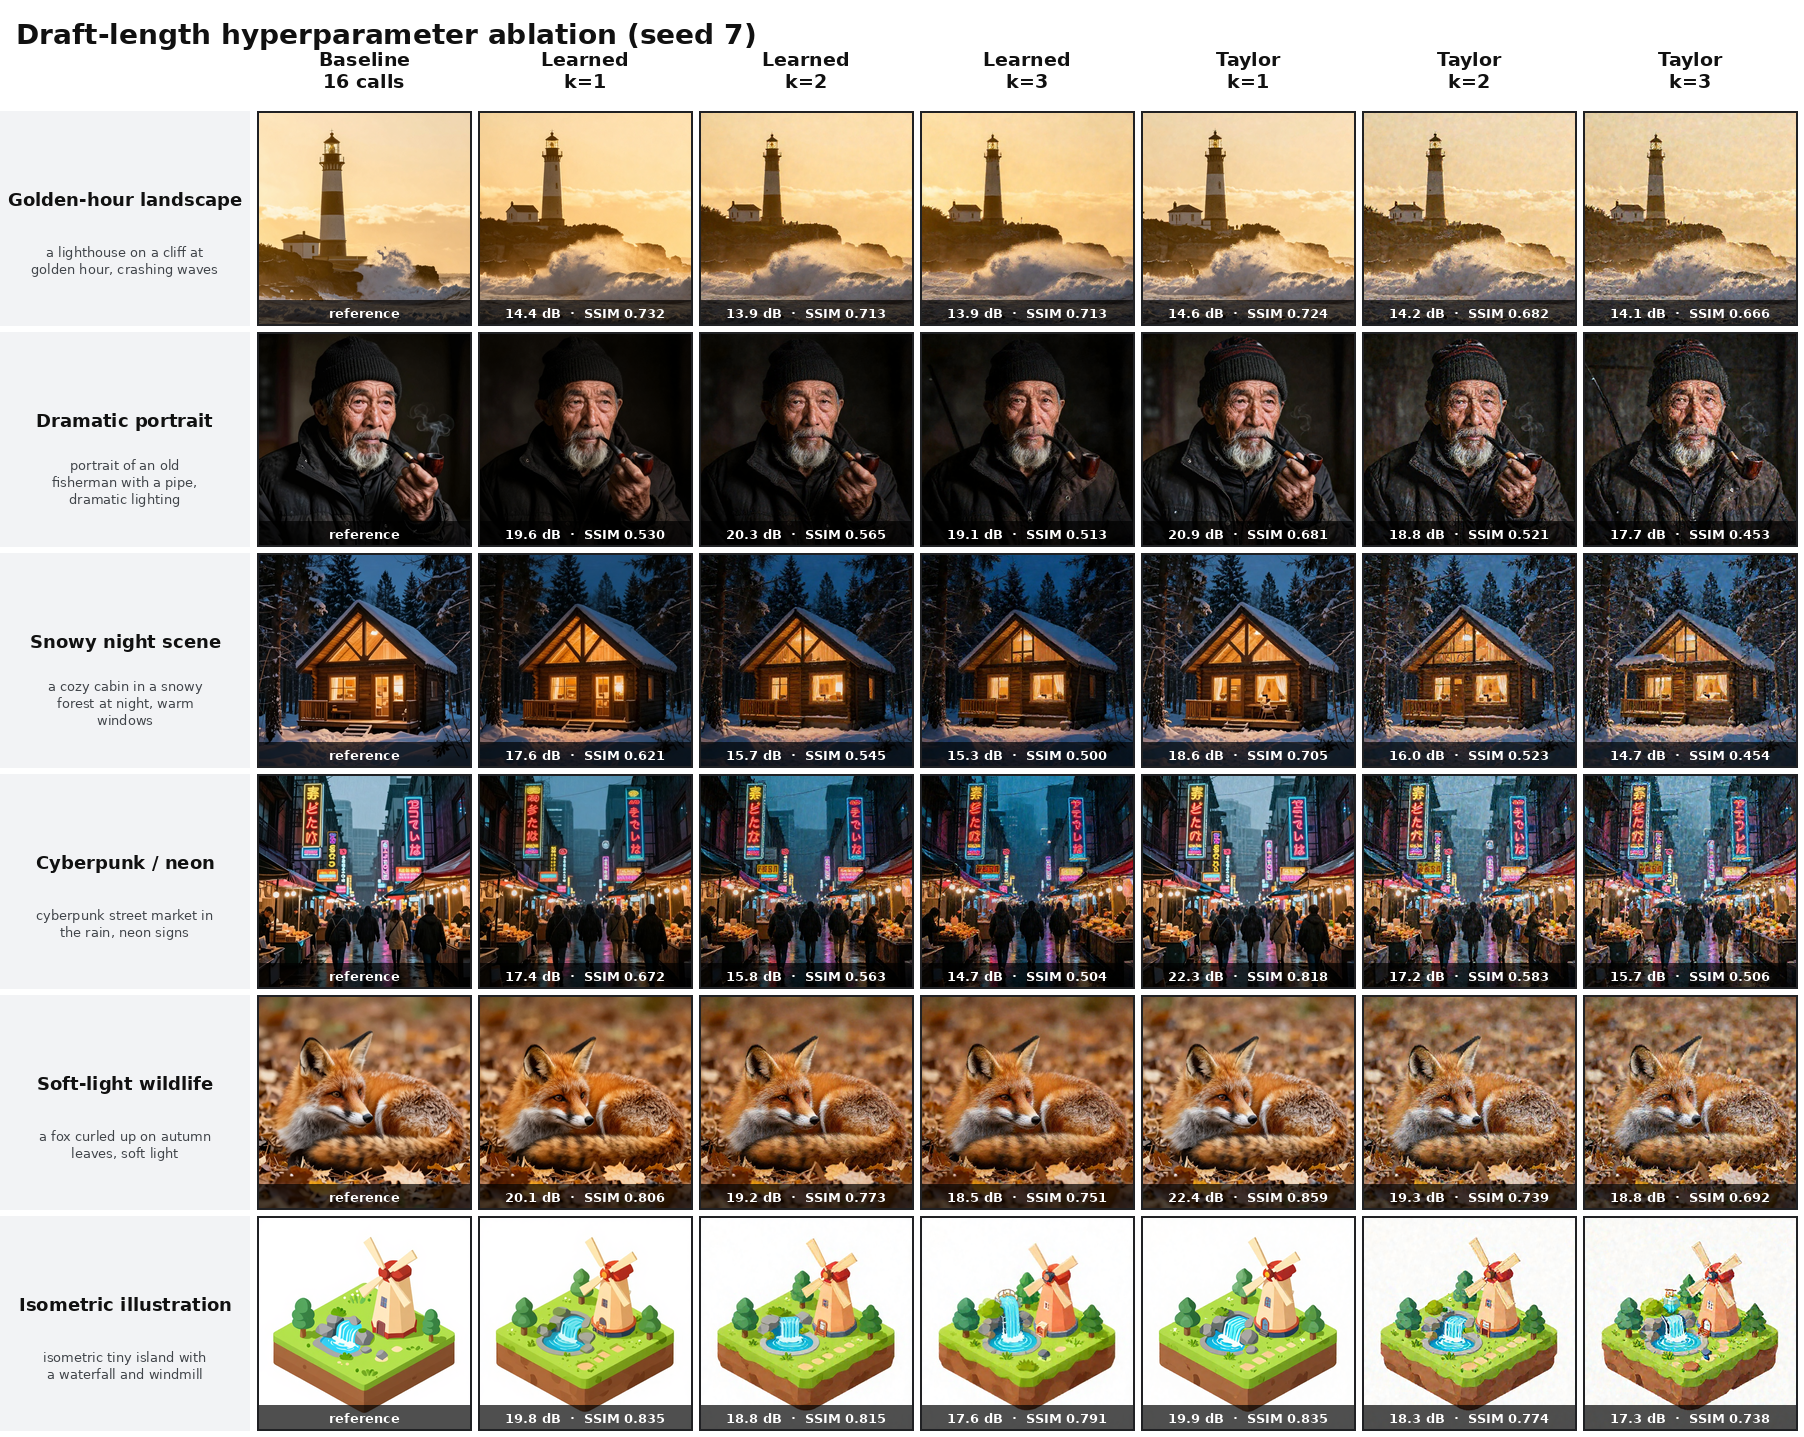
\includegraphics[width=\textwidth]{figures/draft_length_grid.png}
\caption{Draft-length hyperparameter ablation. Columns vary forecaster family
and $k\in\{1,2,3\}$; rows vary prompt/style slice. Increasing $k$ means fewer
real denoiser calls (9, 6, and 5 respectively) and progressively greater
departure from the same-seed reference. Panel labels report PSNR and SSIM.}
\label{fig:draft-grid}
\end{figure}

\begin{figure}[p]
\centering
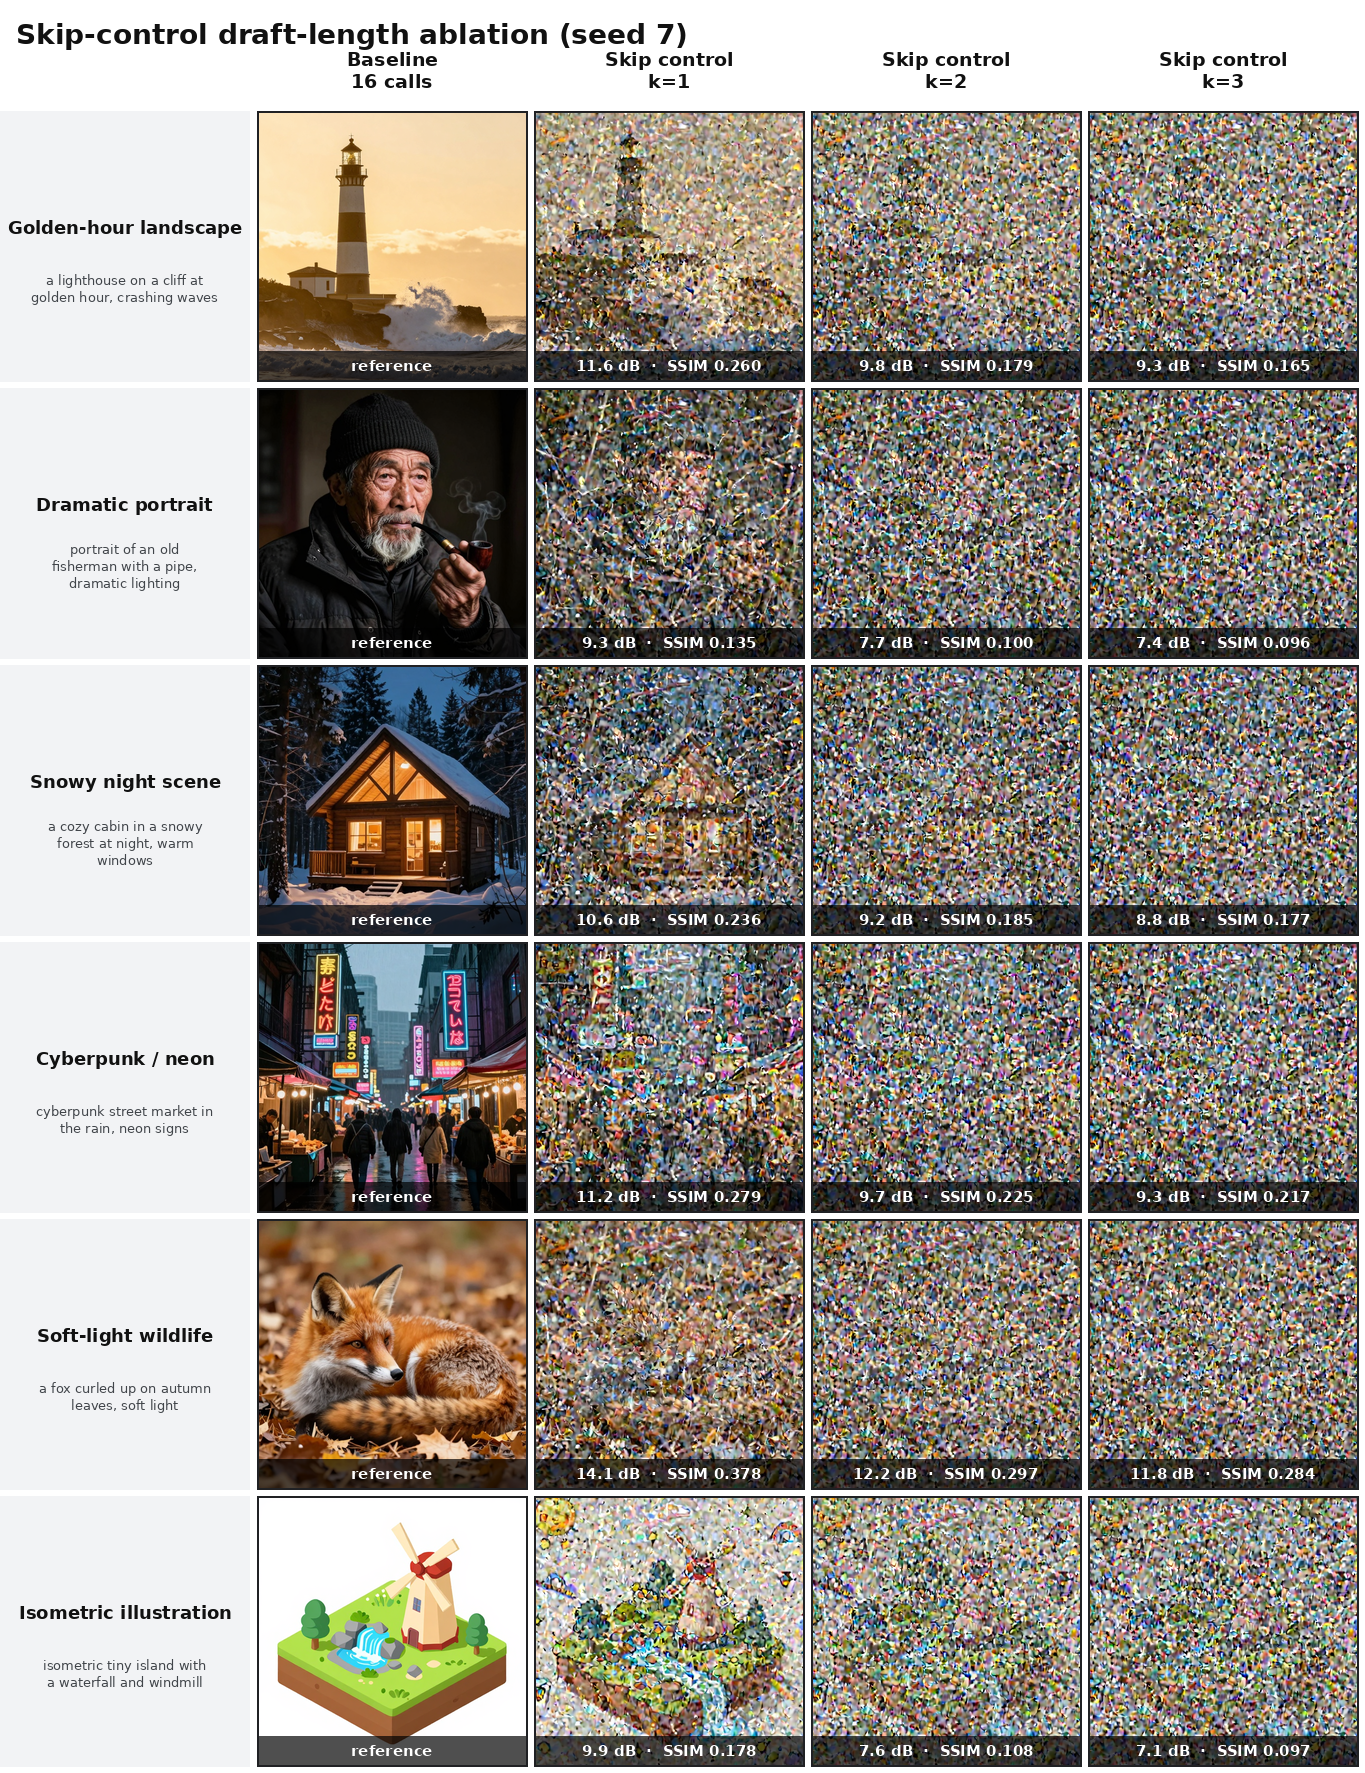
\includegraphics[width=\textwidth]{figures/skip_length_grid.png}
\caption{Skip-control hyperparameter ablation. This arm performs the same real
denoiser-call schedules as the learned and Taylor arms but supplies no latent
correction. Its outputs deteriorate from weak structure at $k=1$ to coloured
noise at $k=3$, demonstrating that call removal alone does not yield a viable
sample.}
\label{fig:skip-grid}
\end{figure}

\subsection{A correction to our own earlier numbers}
\label{sec:correction}

Our first analysis of these runs reported a mean speedup of
$\ReportedSpeedupKThree\times$ at $k=3$. That number is wrong, and the way it was
wrong is instructive.

The harness times the baseline arm first, for each prompt, with no warm-up
iteration. The first baseline call therefore absorbs CUDA context creation,
cuBLAS/cuDNN autotuning and lazy module initialisation: it took
$\WarmupBaseline$\,s against a $\MedianBaseline$\,s median for identical work.
Because speedup is computed as $t_\text{baseline}/t_\text{method}$ per prompt and
then averaged, that single contaminated row contributed a spurious
$3.79\times$ and carried the mean. The same pattern appears at $k=1$ ($96.8$\,s)
and $k=2$ ($64.1$\,s), inflating those means too.

Excluding rows whose baseline exceeds twice the median --- the rule our analysis
script now applies and reports --- the means fall to the values in
Table~\ref{tab:e2e}. We record this because a $1.5\times$ claim and a
$1.04\times$ measurement lead to different engineering decisions, and because
the failure is entirely generic: any benchmark that times a cold arm first and
averages ratios will do this.

\section{Recommendations}

The ablations define a focused next tuning loop.

\begin{enumerate}
  \item \textbf{Tune from the Taylor $k=1$ reference.} It is the best measured
    speed/retention point: $\SpeedupTaylorKOne\times$ at
    $\PsnrTaylorKOne$\,dB PSNR, with no learned checkpoint or extra model
    allocation.
  \item \textbf{Promote schedule-calibrated momentum into the next image
    sweep.} Its five-fold trajectory error is 20--33\% below raw Taylor and it
    captures nearly all of the benefit of the more complex two-delta fit. Test
    it at $k=1,2,3$ with the same seeds before claiming an image-level gain.
  \item \textbf{Align learned training with the output metric.} Save the best
    validation checkpoint and add decoded perceptual or preference supervision;
    the present relative-L2 objective improves latent error without beating the
    Taylor image baseline.
  \item \textbf{Treat routing as a second-stage optimisation.} The
    reference-aware oracle adds at most 0.38 dB in this sweep, so a router has
    less immediate headroom than improving the forecaster itself.
  \item \textbf{Test removal of the final step for this exact schedule.} The
    stored float16 trajectory duplicates its final latent. Gate the optimisation
    on a runtime equality/tolerance check rather than generalising it to other
    schedulers or step counts.
  \item \textbf{Report denoiser-only and end-to-end timing together.} Warm up
    every arm, cache prompt embeddings where the serving workload permits it,
    and separate sampling from VAE decode. This reveals both the method gain and
    the user-visible gain.
  \item \textbf{Expand the operating-point grid} to higher resolution, longer
    or undistilled schedules, and batches greater than one. Those settings give
    saved denoiser calls enough share of total time to matter.
\end{enumerate}

\section{Serving Integration}

The intended deployment target is a single-GPU multi-tenant server in which a
diffusion worker shares a device with a language model, a background-removal
worker and a 3D worker. Two pieces of that stack are relevant here and are open
source \citep{omniservenative}.

First, admission and device-memory arbitration. Four processes sizing their own
workloads from \texttt{cudaMemGetInfo} is a race: the read counts a caching
allocator's retained blocks as used, and is stale the instant two tenants read
it concurrently, so both size a batch against the same free bytes and the second
runs out of memory. The gateway replaces this with a lease broker --- a tenant
asks for headroom and is told a number it may rely on, with granted-but-not-yet
allocated memory withheld from the next caller. This is what would allow a draft
model to be resident at all, which is the natural next step for the speculative
family.

Second, the request path itself is C rather than Python, with the HTTP relay
preserving byte-exact streaming so that image bytes are never re-encoded.
CuteDSL contributes fused kernels used by the Z-Image transformer on sm\_120 ---
fused QKV projection with RoPE, fused QK-norm, RMS norm, SiLU-gated FFN and
AdaLN --- which accelerate the denoiser itself and are therefore complementary to
everything in this paper: they make each step cheaper, whereas we tried to make
steps fewer. Given the Amdahl result of Section~\ref{sec:e2e}, kernel work of
this kind is currently the better investment of the two at our operating point.

\section{Limitations and Threats to Validity}
\label{sec:limitations}

\paragraph{The base model is already distilled.} Z-Image Turbo is a few-step
model. Step-reduction methods have far less to remove from an already-compressed
schedule than from a 50-step sampler, and results here should not be
extrapolated to undistilled checkpoints, where we would expect drafting to look
considerably better.

\paragraph{Small prompt and seed set.} Six prompts per configuration, one seed,
and five prompts after warm-up exclusion for timing. The contact sheets expose
every image rather than hiding this sample size, but they do not turn six
examples into a population. This is enough to establish that the timing effect
is near $1.0\times$ and nowhere near enough to rank methods separated by a few
percent. The method-by-style reversals at $k=3$ are evidence against a universal
ranking, not evidence for six distinct style distributions.

\paragraph{PSNR and SSIM are retention metrics, not quality judges.} A drafted
trajectory that lands on a different but equally plausible image is penalised as
heavily as one that lands on mush. The qualitative artifacts show precisely
this: many drafted images remain recognisable while differing compositionally
from the baseline, whereas the skip arm's $8.9$\,dB correctly identifies noise.
SSIM adds structural sensitivity but inherits the same reference dependence. A
perceptual or preference-based metric is needed, and a visual-ranking model ---
for instance the Gemma model already resident in the serving stack, used as a
pairwise judge --- is one possible instrument. We have not run this, and we
decline to report an aesthetic-quality ranking we have not measured.

\paragraph{The trajectory cache is not evaluated end-to-end here.} The
predictability and drafting results are measured; the $k$-NN teleportation
results are not included in this report, and the production trajectory corpus
(3D assets and an art library, on the order of tens of gigabytes) is
described from the system design rather than measured in these experiments.

\paragraph{No exact verification.} Unlike speculative decoding, our accepted
latents are not guaranteed to match the target model's. Every method here trades
quality for time, and the confidence gate bounds that trade heuristically rather
than provably.

\section{Conclusion}

Latent teleportation is a family of approximate trajectory forecasts and warm
starts for diffusion, not an exact verifier. The premise is supported: the
trajectory is smooth enough that one schedule-calibrated momentum scalar reduces
held-out forecast error by 20--33\% over raw Taylor, and the evaluated drafting
schemes remove up to $\CallReductionKThree\times$ denoiser calls. All 36 learned
and Taylor candidates in the image sweep preserve the requested subject or
scene, while larger horizons introduce visible retention costs that the grids
make explicit.

At the tested $512^2$/16-step serving point, fixed text and VAE work masks most
of the saved calls: speculative walking measures $\CorrectedSpeedupKThree\times$
end to end and the destructive skip ceiling is
$\CorrectedSkipKThree\times$. That result identifies where the system must move
next. The immediate milestone is to run schedule-calibrated momentum through
the full image sweep, measure denoiser-only timing alongside end-to-end timing,
and repeat at operating points where denoising dominates. Cache-guided
teleportation, confidence gating, and LoRA-space transport then remain distinct
follow-on hypotheses rather than implied results.

The corrected warm-up analysis is equally important: the apparent
$\ReportedSpeedupKThree\times$ became $\CorrectedSpeedupKThree\times$ when a
cold first iteration was removed. Publishing both the promising forecasting
signal and the actual serving constraint gives future tuning a reliable
baseline.

\subsubsection*{Reproducibility}

Code, both analysis harnesses, generated contact sheets, their source hashes,
and the raw summary JSON are in \citet{cutedsl}. Full-resolution source panels
remain in the experiment store; the committed grids contain every panel used in
the paper. The serving gateway is in
\citet{omniservenative}. The LoRA adapter library is not open source; its
integration mechanism is described in Section~\ref{sec:lora}.

\bibliography{refs}

\end{document}
